\documentclass{article}
\usepackage[utf8]{inputenc}
\usepackage[T1]{fontenc}
\usepackage[english]{babel}
\usepackage{hyperref}
\usepackage{graphicx}
\usepackage{float}
\graphicspath{{img/}}

\title{My Report}
\author{Your Name}
\date{\today}

\begin{document}

\maketitle

\newpage
\tableofcontents
\newpage

\section{Introduction}
Provide an overview of the internship, its context, and main objectives.

\section{Data Preparation}
The first step is to find the public data available on the subject, to understand and explore it, and to prepare it for analysis.

\subsection{Databases}
In France, the water quality legally obligated to be monitored, with measurements being taken regularly all over the country.
Theses measurements takes place at different stages of the water treatment process, and are stored in several databases.

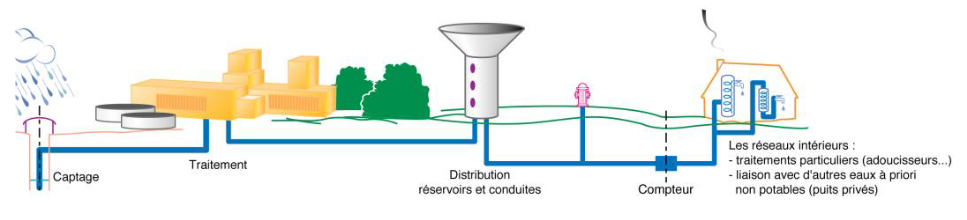
\includegraphics[width=0.8\textwidth]{Process_eau.png}

The following databases contains theses measurements, and are all maintained aswell as publicly accessible online.
\begin{itemize}
    \item \textbf{Source Water Quality} -- (\href{https://www.data.gouv.fr/fr/datasets/resultats-du-controle-sanitaire-de-leau-distribuee-commune-par-commune/}{Measurements taken at the source, whether groundwater or surface water})\footnote{\url{https://www.data.gouv.fr/fr/datasets/resultats-du-controle-sanitaire-de-leau-distribuee-commune-par-commune/}}
    \item \textbf{Sanitary Control of Distributed Water} -- (\href{https://www.data.gouv.fr/fr/datasets/resultats-du-controle-sanitaire-de-leau-du-robinet/}{Measurements taken at the water treatment centers, before distribution})\footnote{\url{https://www.data.gouv.fr/fr/datasets/resultats-du-controle-sanitaire-de-leau-du-robinet/}}
    \item \textbf{Sanitary Control of Tap Water} -- (\href{https://ades.eaufrance.fr/Recherche/Index/QualitometreAvance?g=9220e3}{Measurements taken at random taps within the distribution network})\footnote{\url{https://ades.eaufrance.fr/Recherche/Index/QualitometreAvance?g=9220e3}}
\end{itemize}
All of theses are also available via the (\href{https://hubeau.eaufrance.fr/}{Hubeau API})\footnote{\url{https://hubeau.eaufrance.fr/}}.

\newpage
\subsection{SANDRE Referentials}
All data related to water quality in France is organized according to the SANDRE (Service d’Administration Nationale des Données et Référentiels sur l’Eau) framework. SANDRE is a national authority responsible for establishing and maintaining standardized reference systems for all aspects of water data, including water sources, treatment facilities, distribution networks, and the parameters used to assess water quality.

The SANDRE referential ensures that every parameter relevant to water quality is assigned a unique identifier, known as \texttt{cdparametre}. This code allows for the unambiguous identification of each measured element—whether it is a physical, chemical, or biological parameter—across all datasets.

The referential is publicly accessible, and SANDRE provides an access to theses referential, as a database of an API, on it's (\href{https://www.sandre.eaufrance.fr/v2/}{website}\footnote{\url{https://www.sandre.eaufrance.fr/v2/}}. It plays an essential role in managing the afformentioned databases.

\subsection{Legislation}
We're also looking for the specific legislation that defines the water potability or not.
The French and European legislation diverges, on the number of parameters included, and on their thresholds aswell.

The specific legislation can be found in the following links:
\begin{itemize}
    \item \href{https://www.legifrance.gouv.fr/loda/id/JORFTEXT000000274485/2022-11-28/}{\textbf{French Legislation on Drinking Water}}\footnote{\url{https://www.legifrance.gouv.fr/loda/id/JORFTEXT000000274485/2022-11-28/}}
    \item \href{https://eur-lex.europa.eu/FR/legal-content/summary/drinking-water-essential-quality-standards.html}{\textbf{European Legislation on Drinking Water}}\footnote{\url{https://eur-lex.europa.eu/FR/legal-content/summary/drinking-water-essential-quality-standards.html}}
\end{itemize}

Theses legislations define the maximum allowed values for microbiological parameters (the presence of dangerous organisms), aswell as chemical parameters.
The full list of chemical parameters criterias is available in the annex.



\subsection{Data Selection}


For the purposes of this internship, we chose to focus our efforts on the \textbf{Sanitary Control of Distributed Water} database. 
This dataset is what is being used to determine the potability of water in each municipalities, which is the subject of our project.
We will of course make extensive use of the SANDRE database itself to naviguate and process the data. 

\newpage
\subsection{Data Cleaning}
The data cleaning phase is essential to reduce the size of the dataset, which approximate 15Gb in total.
All data sources were provided in CSV format, but with differing delimiters and encoding schemes, and in multiple tables, orginized by years.
We decided to merge all the tables into a single table, dividing it into multiple, one per parameter to keep the memory usage manageable.
The SANDRE referential was reduced to the selected parameters only, aswell as the key values, being the name, the units and the description of the parameter.


\section{Data Exploration}

\subsection{Sandre Parameters}
SANDRE provides an extensive list of parameters, some of which are not relevant to our analysis, and some that are not even measured in the dataset.

Parameters fall into two main types: those with continuous values for every measurement (e.g., temperature), 
and thoses that measure the potential presence of it, which only occasionally yield a non-zero value (e.g., the presence of a contaminant).
Theses 2 types are important to distinguish, as they require different analysis methods.

An important focus on sample size is also nescessary, both geographically and temporally.

So, we decided on 4 filters to determine the parameters to keep:
\begin{itemize}
    \item \textbf{Temporal Sample Size}: The average number of measurements of the parameter for each commune.
    \item \textbf{Geographical Sample Size}: The number of communes where the parameter is measured.
    \item \textbf{\% non-zero values}: The percentage of non-zero measurements of the parameter. Used to determine the type of numerical data.
\end{itemize}

We processed the entire dataset to obtain theses factors for each parameter, and 

We obtained the following parametesr, of which, only X are present in the legislation:
\begin{itemize}
    \item Température de l'Eau
    \item Potentiel en Hydrogène (pH)
    \item Conductivité à 25°C
    \item Hydrogénocarbonates
    \item Chlorures
    \item Sulfates
    \item Nitrates
    \item Dureté totale
    \item Titre alcalimétrique complet (T.A.C.)
    \item Potassium
    \item Magnésium
    \item Calcium
    \item Sodium
    \item Chlore libre
    \item Chlore total
    \item Carbone Organique
    \item Equilibre calcocarbonique de l’eau destinée à la consommation humaine
    \item Nitrates/50 + Nitrites/3
    \item Température de mesure du pH
    \item pH d'equilibre
    \item Fluorure anion
\end{itemize}

\newpage
\section{Analysis Methods}
We performed a compre3hensive analysis of the water quality data, focusing on both geographical and temporal aspects.

\subsection{Temporal Analysis}

First and foremost, for any temporal analysis, we first need a preprocessing of the data, to de-regionalize the measurements, allowing for a broader analysis of the parameters.
This involves several steps for each parameter:
\begin{itemize}
    \item Center-reducing all measurements by the commune mean and standard deviation.
    \item Aggregating The data.
    \item Removing outliers, defined as values outside 3 standard deviations from the centered reduced mean (0), and standard deviation (1).
    \item Smoothing the data using a 60-day rolling window to reduce noise.
    \item Re-adding the global mean and standard deviation to the data.
\end{itemize}

Because we need the mean and standard deviation by commune, this implies a decent sample size for each communes.
Thus we filter out the communes with less than X measurements for each parameter.
We can now perform a series of timeseries analyses, including:
\begin{itemize}
    \item Linear regression to identify trends over time.
    \item Fourier analysis to detect seasonal patterns and periodicities in the data.
\end{itemize}

From this, we can identify the seasonal parameters, such as temperature, or more indirectly, the pH.

\subsection{Correlation Analysis}
Correlation analysis for timeseries aims to identify relationships between different parameters, 
particularly over time. For time series data, we compute Pearson correlations, which can detect correlations with a lag.
However, strong correlations can arise simply due to shared seasonality or trends. 
To obtain meaningful results, it is essential to detrend and deseasonalize 
the data before calculating correlations, ensuring that observed relationships 
reflect genuine interactions rather than coincident temporal patterns.
We also need a centered reduced and de-regionalized data, as described in the previous section.

Note that making a correlation matrix requires a significant amount of memory,
since we have to process all possible pairs of parameters.
There was a significant effort toward optimizing the memory usage, as per the annex X.

\subsection{Potability Index}
We want to check if the water quality is up to the european and french standards.
To do so, we mapped each communes green if no measurement exceeded the legal limit, 
and a shade between yellow and red for the percentage of measurements that exceeded the legal limit.

\section{Results}
For the moment, we only focused on the Charente-Maritime department, and the Sanitary Control of Distributed Water database.


\subsection{Potability Index Results}


\section{Future Work}
Suggest possible directions for future research and improvements.

\section{Conclusion}
Summarize the key findings and contributions of the internship.

\appendix
\section{Annex}

\subsection{List of Acronyms}
\begin{itemize}
    \item SANDRE: Service d’Administration Nationale des Données et Référentiels sur l’Eau
    \item API: Application Programming Interface
    \item CSV: Comma-Separated Values
    \item T.A.C.: Titre Alcalimétrique Complet
\end{itemize}

\subsection{Example of Data Structure}
\begin{verbatim}
| Date       | Commune   | cdparametre | Value | Unit  |
|------------|-----------|-------------|-------|-------|
| 2023-01-01 | Paris     | 1234        | 7.2   | pH    |
| 2023-01-01 | Lyon      | 5678        | 0.05  | mg/L  |
\end{verbatim}

\subsection{Useful Links}
\begin{itemize}
    \item \url{https://hubeau.eaufrance.fr/}
    \item \url{https://www.sandre.eaufrance.fr/}
    \item \url{https://www.data.gouv.fr/}
    \item \url{https://eur-lex.europa.eu/FR/legal-content/summary/drinking-water-essential-quality-standards.html}
\end{itemize}

\subsection{Summary Table: French vs European Criteria}
\begin{table}[H]
\centering
\begin{tabular}{|l|l|l|l|}
\hline
\textbf{Code} & \textbf{Substance} & \textbf{French Limit} & \textbf{European Limit} \\
\hline
1376 & Antimoine & 5,0 µg/l & 10 µg/l \\
1369 & Arsenic total & 10 µg/l & 10 µg/l \\
1396 & Baryum & 1,0 mg/l & -- \\
1362 & Bore & inf mg/l & 1,5 mg/l \\
1388 & Cadmium & 3,0 µg/l & 5,0 µg/l \\
1389 & Chrome & 50 µg/l & 25 µg/l \\
1392 & Cuivre & 1,0 mg/l & 2,0 mg/l \\
1390 & Cyanures & 70 µg/l & 50 µg/l \\
7073 & Fluorures & 5,0 mg/l & 1,5 mg/l \\
1382 & Plomb & 10 µg/l & 5 µg/l \\
1394 & Manganèse & 500 µg/l & -- \\
1387 & Mercure & 1,0 µg/l & 1,0 µg/l \\
1386 & Nickel & 20 µg/l & 20 µg/l \\
1340 & Nitrates & 50 mg/l & 50 mg/l \\
1339 & Nitrites & 0,1 mg/l & 0,50 mg/l \\
1385 & Sélénium & 10 µg/l & 20 µg/l \\
1457 & Acrylamide & -- & 0,10 µg/l \\
1114 & Benzène & -- & 1,0 µg/l \\
1115 & Benzo(a)pyrène & -- & 0,010 µg/l \\
2766 & Bisphénol A & -- & 2,5 µg/l \\
1751 & Bromates & -- & 10 µg/l \\
1752 & Chlorates & -- & 0,25 mg/l \\
1735 & Chlorites & -- & 0,25 mg/l \\
1161 & 1,2-dichloroéthane & -- & 3,0 µg/l \\
X & Épichlorhydrine & -- & 0,10 µg/l \\
X & Acides haloacétiques (AHA) & -- & 60 µg/l \\
2058 & Microcystine-LR & -- & 1,0 µg/l \\
X & Pesticides & -- & 0,10 µg/l \\
6276 & Total pesticides & -- & 0,50 µg/l \\
X & Total PFAS & -- & 0,50 µg/l \\
8847 & Somme PFAS & -- & 0,10 µg/l \\
X & Hydrocarbures aromatiques polycycliques & -- & 0,10 µg/l \\
2963 & Tétrachloroéthylène et trichloroéthylène & -- & 10 µg/l \\
2036 & Total trihalométhanes & -- & 100 µg/l \\
1361 & Uranium & -- & 30 µg/l \\
1753 & Chlorure de vinyle & -- & 0,50 µg/l \\
\hline
\end{tabular}
\caption{Summary Table: French vs European Criteria for Drinking Water}
\end{table}

\end{document}